
\documentclass[%
 reprint,
%superscriptaddress,
%groupedaddress,
%unsortedaddress,
%runinaddress,
%frontmatterverbose, 
%preprint,
%showpacs,preprintnumbers,
%nofootinbib,
%nobibnotes,
%bibnotes,
 amsmath,amssymb,
 aps,
% draft,
%pra,
%prb,
%rmp,
%prstab,
%prstper,
%floatfix,
]{revtex4-1}
%\usepackage{biblatex}
\usepackage{graphicx}% Include figure files
\usepackage{dcolumn}% Align table columns on decimal point
\usepackage{bm}% bold math
\usepackage{xspace}
\usepackage{float}
%\usepackage[showframe]{geometry}% http://ctan.org/pkg/geometry
\usepackage{lipsum}% http://ctan.org/pkg/lipsum
\usepackage[export]{adjustbox}
\usepackage{gensymb}
\usepackage{newunicodechar}
\usepackage[utf8]{inputenc}
\usepackage[table]{xcolor}
\usepackage{graphics}



 
%\usepackage{hyperref}% add hypertext capabilities
%\usepackage[mathlines]{lineno}% Enable numbering of text and display math
%\linenumbers\relax % Commence numbering lines

%\usepackage[showframe,%Uncomment any one of the following lines to test 
%%scale=0.7, marginratio={1:1, 2:3}, ignoreall,% default settings
%%text={7in,10in},centering,
%%margin=1.5in,
%%total={6.5in,8.75in}, top=1.2in, left=0.9in, includefoot,
%%height=10in,a5paper,hmargin={3cm,0.8in},
%]{geometry}


\begin{document}

%\preprint{APS/123-QED}
\newunicodechar{°}{\degree}
\newcommand {\gr}{$\gamma-ray$\xspace}
\newcommand {\grs}{$\gamma-rays$\xspace}
\newcommand {\gp}{$\gamma_{\text{photon}}$\xspace}
\newcommand {\cs}{$^{137}$Cesium \xspace}
\newcommand {\ba}{$^{133}$Barium \xspace}
\newcommand {\co}{$^{60}$Cobalt \xspace}
\newcommand {\na}{$^{22}$Sodium \xspace}
\newcommand {\fp}{\textit{findpeaks}\xspace}
\title{Excitation and Ionization Energies of Helium and Mercury}% Force line breaks with \\


\author{Lee Allers, Lucas Thoennes}

\date{\today}% It is always \today, today,
             %  but any date may be explicitly specified

\begin{abstract}
\begin{center} \textbf{Abstract}\end{center}
%\begin{description}
%\item[Usage]
%Secondary publications and information retrieval purposes.
%\item[PACS numbers]
%May be entered using the \verb+\pacs{#1}+ command.
%\item[Structure]
%You may use the \texttt{description} environment to structure your abstract;
%use the optional argument of the \verb+\item+ command to give the category of each item. 
%\end{description}
By exploring how adding energy to an atomic or molecular system using elastic and inelastic collisions of electrons into the system, we find quantized energy levels, as predicted by the \textit{ Bohr Model} \cite{bohrmodel},  that provide a unique signature of that atom. By exploring these quantized energy levels of Helium and Mercury through these collisions, we're able to define atoms simply by their excitation/ionization profile. This allows us to probe deeper into into the structure of the larger macroscopic systems to define their atomic compositions, among other things. This has practical applications in all of science: It allows chemists to find the properties of an unknown system, Analysis of Biological fluids, Forensic Applications, Mass Spectrometry, etc.
\end{abstract}

%\pacs{Valid PACS appear here}% PACS, the Physics and Astronomy
                             % Classification Scheme.
%\keywords{Suggested keywords}%Use showkeys class option if keyword
                              %display desired
\maketitle

%\tableofcontents

%\begin{figure}[ht!]
%\includegraphics[width = .5\textwidth ,keepaspectratio,frame]{spec.jpg}
%\caption{ The gamma-ray spectrum of natural uranium, showing about a dozen discrete lines superimposed on a smooth continuum, \\
%allows one to identify the nuclides of the uranium decay chain.\cite{WS}}
%\end{figure}
%\begin{figure}[!ht]

%\includegraphics[width = .5\textwidth ,keepaspectratio,frame]{PMT.jpg}
%\caption{ Schematic of a photomultiplier tube coupled to a scintillator. This arrangement is for detection of gamma rays.\cite{Sim} The various parts are discussed in further detail in the %Theory and methods section of this paper.}
%\end{figure}

\section{\label{sec:level1}Introduction}
\begin{figure}
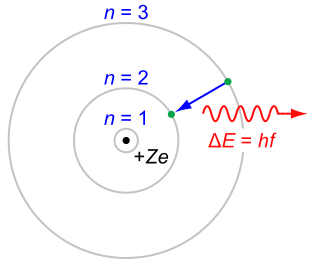
\includegraphics[width = 6cm,keepaspectratio]{bohrmodel.png}
\caption{Bohr Model of the hydrigen atom where n is the principal quantum number, Z is the proton number, e is the electron charge, $\Delta E$ is the change in energy, h is plancks constant, and f is the frequency. The 3 $\rightarrow$ 2 transition depicted here produces 
the first line of the Balmer series, and for hydrogen (Z = 1) it results in a photon of wavelength 656 nm (red light).\cite{bohrmodel} }
\end{figure}

In 1913,  Neils Bohr and Ernest Rutherford published the \textit{Rutherford-Bohr Model}\cite{bohrmodel}\textbf{Fig. 1}, henceforth referred to as the Bohr Model. This was a highly simplified model of the Hydrogen atom and required quantum mechanics to later become much more accurate. However, the Bohr Model gives us an simple way to understand the energy levels in an atom and revolutionized the idea of atoms having quantized energy states. The Bohr Model \cite{bohrmodel} turned out to be incorrect, due to the underpinning quantum mechanics not known when he derived the model, but was still useful to predicted energies in idealized situations of the Hydrogen atom to a first-order approximation.This allowed Bohr to formulate the following relation,
\[ \Delta E = E_f - E_i \]
where $E_f$ is the final energy, $E_i$ is the initial energy,
\[ E = h\nu \]

where h is planck's constant, and $\nu$ is the frequency. \\
Eventually, the energy relation to quantum number $n$ to discrete energy levels in the atom, lead to the equation
\[
E_n = -\frac{m_e Z^2 e^4}{8\epsilon_0^2 h^2n^2}eV
\]
\begin{equation}\label{eq:qe}
E_n = -13.6(\frac{Z^2}{n^2})\quad eV
\end{equation}
where $m_e$ is the mass of the electron, $Z$ is the proton number, $e$ is the electron charge, $\epsilon_0$ is the permitivity of free space constant, $h$ is plancks constant, and $n$ is the principal quantum number. A more formal derivation of this equation can be found at citation\cite{esderiv}. This allows us to predict energies of idealized atoms which are often termed `hydrogen-like' (one electron). However, it's more complicated for Helium and Mercury. Bohr's model showed us that an electron with less energy than is required to excite an atom from it's ground state to the excited state can not take place. What we expect to see theoretically is pictured in \textbf{Fig. 2} where the four different excitation levels are pictured as an excitation from the ground state to the first excited state 2s,2p singlet and $2^3s$,$2^3p$ triplet \cite{hell} , where the singlet state has a net angular momentum, $s = 0$ and the triplet state has a net angular momentum of $s = 1$\cite{hell}. We also explore the regime of energy where Ionization of the atom takes place, that is, where there is enough energy in the incident electron to remove the outer electron completely from the atom. In \textbf{Fig. \ref{fig:helex}} we see a spectroscopic model of how these energy states transition in Helium, where n is the integer number corresponding to the principal quantum number and ~24.6 eV is the Ionization energy for Helium. Although there is an Ionization energy for Mercury, we will not reach the energies required to view this process.

\begin{figure}
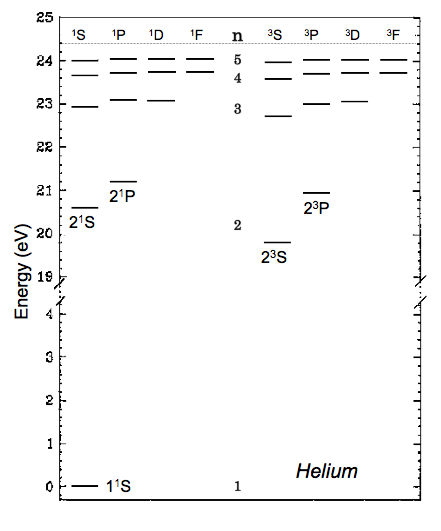
\includegraphics[width = 6cm,keepaspectratio]{ee.png}
\caption{Helium excitation levels from 1s to 2s,2p singlet and $2^3s$,$2^3p$ triplet states.\cite{hell}}
\label{fig:helex}
\end{figure}


This gives us clear direction to explore the properties of both Helium and Mercury. To measure these excitation energies, we use equipment that allows us to measure the current generated by inelastic collisions of electrons onto helium and mercury gases, where the energy of the electrons are absorbed by the atoms in discrete packets, packets being the excitation energy levels. This produces peaks and valleys in the data that correspond to these energy levels. Comparing the theoretical model vs. our data allows us to clearly define whether or not these discrete energy levels exist and how closely our approximation fits the accepted values. Showing these discrete excitation energy levels has many practical applications throughout science; by bombarding atomic and molecular systems with electrons at specific energies, we can develop a model of the atomic structure of these atoms/molecules, because they have discrete signatures. This allows classification of systems that we may not know anything about beforehand.


\section{\label{sec:meth}Methods}
\subsection{\label{sec:hel}Helium}

We begin this experiment by setting up our equipment shown in \textbf{Fig \ref{fig:helb}}. We connect the Filament supply to the helium bulb (in \textcolor{blue}{blue}). The Filament supply provides a heating element to the filament (in \textcolor{red}{red}). The filament is heated and emits electrons through thermionic emissions. The Anode Supply supplies a constant voltage between 0-30V to the control unit. This is set to ~30V to ensure we see all expected peaks of our chosen atom.  The control unit reads the voltage received by the Anode supply and, using Labview software, provides an output voltage to the Anode of the bulb, in discrete voltage steps, 80 mV in our case. This creates an accelerating potential between the Anode and Cathode (in \textcolor{green}{green}) which also ultimately makes a potential on the bulb itself that transfers electrons that collect on the bulb due to only elastic collisions. The electrons are accelerated through this potential and the resultant measurements, current, are from electrons that have lost most of their kinetic energy due to inelastic collisions with the helium gas. These electrons are collected by the collector ring and transmitted through the coaxial cable to the pico-amplifier as a current. An important note is that there is a 1.5V AA Battery connected to this setup. This ensures that the collector ring is at a higher positive potential than the bulb and therefore, will collect only negative charges (from electrons). To view Ionization of helium, we instead reverse the battery to provide a negative potential on the collector ring such that it collects any positively charged ions. The pico-amplifier then amplifies this signal and sends it to the control unit where the final signal is output to Labview as a Current, in arbitrary units.\\

We used two different voltages to gather data and explore the effects and voltage changes. To take data, we run Labview with specific settings, as detailed in the Data section, and find the voltage values of the notable peaks produced. Comparing these peaks to the expected values allows us to determine whether or not the experiment was successful and to what degree. To further ensure that we have enough data, 4 total runs of data are taken with constant Labview parameters at each filament voltage.


\subsection{\label{sec:hel}Mercury}

We begin this experiment by setting up our equipment shown in \textbf{Fig \ref{fig:merb}}. Not pictured here is the AC power supplied to the Mercury apparatus. This AC power supply heats the apparatus to a uniform temperature, specified by the user, 150 and 180 degrees respectively in our case. We heat this apparatus because there is a small bit of Mercury inside that requires heating to produce the mercury vapor. To obtain temperature readings, we insert a thermometer into the apparatus using the access hole on the top. We let the Mercury apparatus heat to a desired temperature, as read on the thermometer, with a variable dial set to 6 in our case, for roughly 15 minutes. We then connect the Filament Supply to the Mercury apparatus. As in the Helium case, this filament supply heats the filament (in \textcolor{red}{red}) inside the apparatus which ejects electrons due to thermionic emission. Again, the Anode Supply supplies a constant voltage to the control unit. The control unit steps the voltage by varying amounts depending on the user's Labview specifications, 80 mv in our case, and supplies that voltage to the Anode (A) of the Mercury Apparatus. The electrons emitted from the filament are accelerated though the potential created by the anode (A) and cathode (K). The 1.5V AA Battery provides a higher positive potential to the collecting electrode (M), where the electrons without enough energy to overcome this potential are ``pushed away'' and re-collected by the cathode of the apparatus. The signal we receive should be from electrons with enough kinetic energy to overcome the collecting electrode's potential. As in helium, this signal is then amplified and output by Labview as a current.

We used two different temperatures to heat the mercury apparatus (not the filament) to gather data about the effects of temperature change in the apparatus. As stated above, to begin taking data we run Labview with specific settings, as detailed in the Data section, and find the values of the excitation peaks produced. Comparing these peaks to the expected value allows us to determine whether or not the experiment was successful and to what degree.

\begin{figure}[!ht]\centering
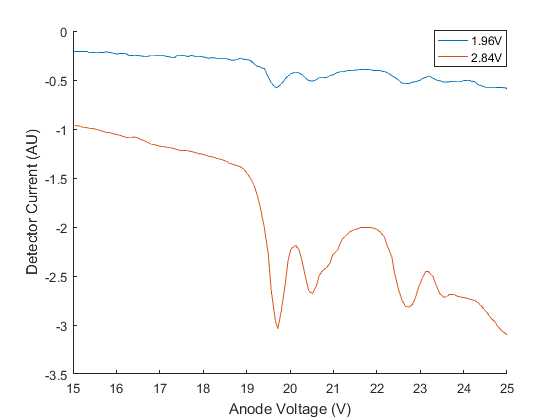
\includegraphics[width = .5\textwidth,keepaspectratio]{fig1.png}
\caption{Plot of Current (in arbitrary units) vs. Supplied anode voltage in steps of 80 mV. Using two sets of data taken by varying the filament supply voltage to be 1.96V (in \textcolor{blue}{blue}) and 2.84V (in \textcolor{red}{red})}
\label{fig:heltwo}
\end{figure}

\section{\label{sec:data}Data}

\subsection{\label{sec:held}Helium}

Using the Labview parameters of \textit{Anode Start Voltage: 10 , Anode End Voltage: 28, Scan Voltage Increment: 80 ,} and \textit{Detector Sensitivity: 5} we find the following plot for the current vs. the voltage, where the anode voltage is increased in increments of 80 mV, \textbf{Fig. \ref{fig:heltwo}}. Because the excitation energy is received by the atom in discrete packets, we expect that changing the voltage to the filament only serves to change the total number of electrons that are emitted and therefore, at a lower/higher filament voltage, we expect to see a smaller/higher current in terms of magnitude, but still having peaks at the same voltages along the x-axis. Note that there are still peaks in the \textcolor{blue}{blue} plot, however, their resolution is diminished when plotted against the higher voltage of 2.84 V.

In \textbf{Fig. \ref{fig:heltworev}} we see the data plots for a reverse biased collector ring. This allows us to see the Ionization energy clearly, as discussed in the analysis section below. In the plot, this is expressed as a sharp increase in the slope of the graph after excitation has taken place.
\begin{figure}[!ht]\centering
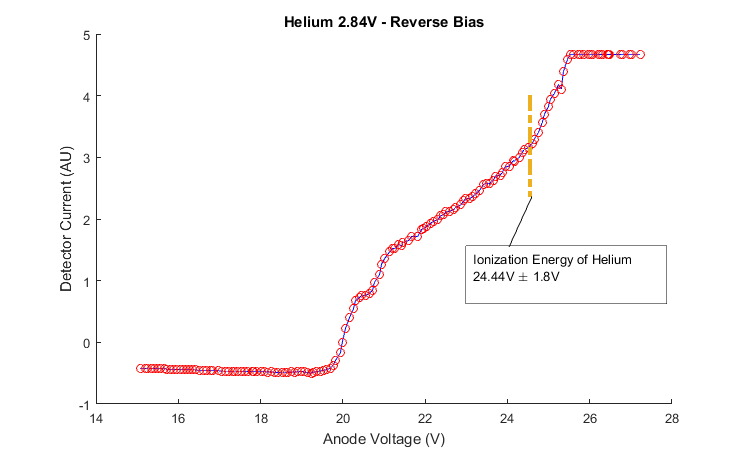
\includegraphics[width = .5\textwidth,keepaspectratio]{fig2.png}
\caption{Plot of Current (in arbitrary units) vs. Supplied anode voltage in steps of 80 mV with the battery reversed to create a negative bias. \textit{as show in \textbf{Fig. \ref{fig:helb}}}}
\label{fig:heltworev}
\end{figure}

\subsection{\label{sec:merd}Mercury}
The mercury data is presented in a plot in \textbf{Fig. \ref{fig:merd}}. We've plotted two different voltages along side two different temperatures. This allows us to analyze how temperature affects the excitation energy. We clearly observe peaks corresponding to each temperature and each voltage variation which is exactly what we expect. The difference between the Helium experiment and this Mercury experiment is that Mercury does not have an apparent ionization energy at these levels. We also observe only a \textbf{total number} of inelastic collisions between the electrons and mercury vapor, i.e the first peak corresponds to, in an idealized case, one electron inelastically colliding with one Mercury atom, the second peak corresponds to, in an idealized case, one electron with enough kinetic energy to have an inelastic collision with two Mercury atoms, and so on.  
\begin{figure}[!ht]\centering
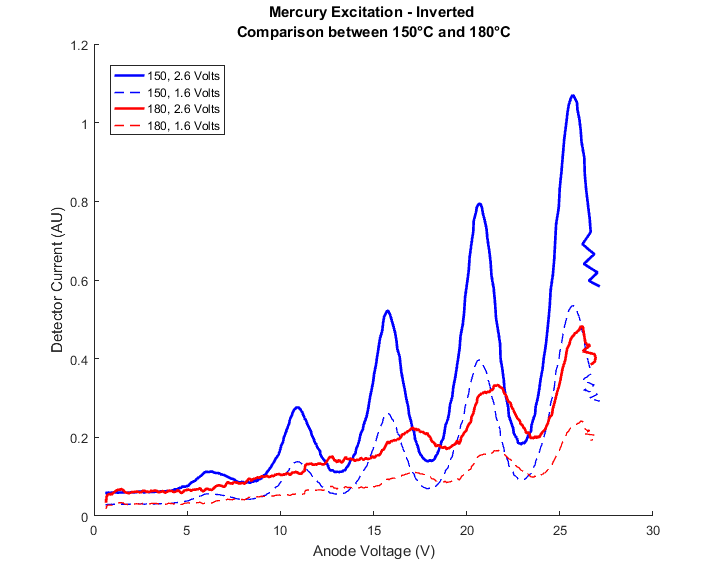
\includegraphics[width = .5\textwidth,keepaspectratio]{22.png}
\caption{Plot of Current (in arbitrary units) vs. Supplied anode voltage in steps of 80 mV. Plot includes data from two different temperatures and with different voltages.}
\label{fig:merd}
\end{figure}

Lastly, as discussed in the \textbf{Methods} section, and being reminded of, changing the temperature of apparatus controls the total amount of Mercury vapor, so we expect to see less electrons able to be received by the collecting electrode because there are more Mercury atoms for the emitted electrons to collide with. This is clearly visible in the data as show by the comparison between the \textcolor{blue}{blue} data and \textcolor{red}{red} data, where the \textcolor{red}{red} data is at a higher temperature and therefore has more mercury atoms in the vapor, takes more Anode Voltage (larger accelerating potential $\rightarrow$ more electron energy) to reach an observable peak in the data. 

\section{\label{sec:data}Analysis}

The equations we'll use throughout the analysis are, finding the mean 
\begin{equation}\label{eq:mean}
\bar x = \frac{1}{N}\sum_{i=1}^N x_i
\end{equation} where $\bar x$ is the expected value and N is the total number of elements of x,
the standard deviation
\begin{equation}\label{eq:std}
\sigma = \sqrt{\frac{1}{N}\sum_{i = 1}^{N}(x - \bar x)^2}
\end{equation} where $\sigma$ is the statistical error. We'll also be combining these methods to find the total error in our experiments where the total error is 

\begin{equation}\label{eq:quad}
\sigma_{final} = \sqrt{\sigma_{stat}^2 +\sigma_{syst}^2} 
\end{equation} where $\sigma_{stat}$ is the statistical error and $\sigma_{syst}$ is the systematic error.
The values we expect to find (listed below) for each experiment are the accepted values today derived over many experiments by many different experimenters,

\begin{center}
\begin{tabular}{ c c}
\begin{tabular}{ |c c| }\hline
\multicolumn{2}{|c|}{Helium}\\
State & Accepted Value\\\hline
Ground State & $0\quad eV$\\
$2^3s$ & $19.8\quad eV$\\
$2^1s$ & $20.61\quad eV$\\
$3^1s$ & $22.90\quad eV$\\
$3^1p$ & $23.21\quad eV$\\
Ionization & $24.6\quad eV$\\\hline
\end{tabular}
 &
\begin{tabular}{ |c c| }\hline
\multicolumn{2}{|c|}{Mercury}\\
&\\\hline
Excitation of & $4.9\quad eV$ \\
&\\
&\\
&\\
&\\
&\\\hline
\end{tabular}
\end{tabular}
\end{center} 

We'll also be using a special Matlab function called \textbf{\textit{findpeaks}}\cite{peak} from the signal processing package, that uses a \textit{quadratic interpolation algorithm}\cite{qi} to find peaks in data, where the prominence parameter is controlled by the user according to experimental requirements. The prominence parameter allows us to set a minimum threshold height for the peaks we wish to observe, ensuring that no extraneous noisy data is included. The \fp function returns values for the FWHM ( width of half of the peak's height), the voltage where the peak occurs, and some other values we will not be using. 

\subsection{\label{sec:helana}Helium}
\begin{figure}[!ht]\centering
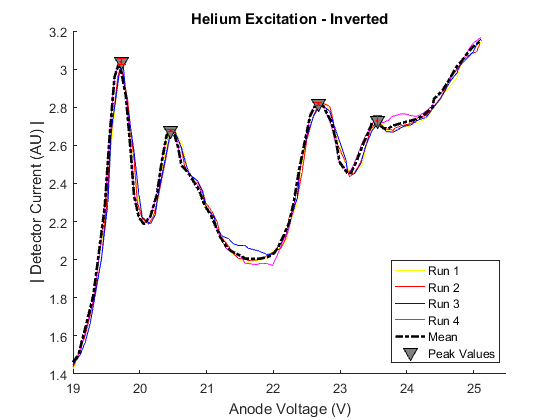
\includegraphics[width = .5\textwidth,keepaspectratio]{peaksinv.png}
\caption{Plot of Current (in arbitrary units) vs. Supplied anode voltage in steps of 80 mV of each experimental run of data, the mean plot of the 4 combined data sets, and the peak locations found.}
\label{fig:peak1}
\end{figure}

For each Filament Voltage, 1.96V and 2.84V respectively, we first find the mean of the peaks, using \textbf{Eq. \ref{eq:mean}}, determined by the \fp function. This also introduces some statistical error in the measurements, given by \textbf{Eq. \ref{eq:std}}.

\begin{center}
\begin{tabular}{c  c  c c }
& Prominence& Peak Voltage & $\sigma_{stat}$\\\hline
1.96 &0.01 & 19.7192 &$\pm$ 0.2001\\
        & &20.5250 &$\pm$ 0.2125\\
        & &22.7960 &$\pm$ 0.1354\\
        & &23.6752 &$\pm$ 0.2441\\\hline
2.48 &0.01 &19.7231&$\pm$0.0800\\
        & &20.4169&$\pm$0.0953\\
        &&22.6548&$\pm$0.1287\\
        &&23.0757&$\pm$0.0258\\ \hline       
\end{tabular}
\end{center}

We chose to take the weighted mean of our experimental data between the two filament voltages used, however, this introduces more statical error since lower voltages mean the data is much more granular. We take the weighted mean by applying the equations

\begin{equation}\label{eq:wm}
\hat x = \frac{\sum_{i = 1}^N (x_i * \sigma_i)}{\sum_{i = 1}^N\sigma_i}
\end{equation}
and error propagation by
\begin{equation}\label{eq:ep} 
\tilde\sigma = \sqrt{\frac{\partial f}{\partial x}\sigma_x^2 + \frac{\partial f}{\partial y}\sigma_y^2 + ...}
\end{equation}

We can also now look at the systematic error from both the resolution of Labview, 80 mV, and the FWHM given by the approximation,
\begin{equation}
FWHM \approx 2.355\sigma
\end{equation} 

To find the final error values we apply \textbf{Eq. \ref{eq:quad}} by taking the known error(s) and adding them in quadrature. Note: Not included in the table below is the statistical error which is shown in the previous table.
\begin{center}
\begin{tabular}{ c  c  c  c }
FWHM & $\sigma_{FWHM}$ &$\sigma_{syst}$  &$\sigma_{final}$ \\\hline
0.32 & 0.1359 & 0.08 & 0.3686\\
0.46 & 0.1953 & 0.08 &0.4420\\
0.46 & 0.1953 & 0.08 &0.4420\\
0.10 & 0.0425 & 0.08 &0.2061 \\\hline 
\end{tabular}
\end{center}
This gives us the total approximated error in our experiment and the final excitation energies. We then compare these to the accepted values of the Excitation energies.
\textbf{
\begin{center}
\begin{tabular}{c  c  c  c }
  Voltage & $\sigma_{final}$ & Accepted Value & \% Difference \\\hline
  19.7203 &$\pm$ 0.3686 & 19.80 & 0.4033 \% \\
 20.4915  &$\pm$ 0.4420 & 20.61 & 0.5765 \%\\
  22.7271 &$\pm$ 0.4631 & 22.90 & 0.7575 \%\\
  23.6178 &$\pm$ 0.2061 & 23.21 & 0.8841 \%\\\hline
\end{tabular}
\end{center}}

These values are in very good agreement with the accepted values for Helium excitation energy levels.\\
If we look back to \textbf{Fig. \ref{fig:heltworev}}, we can use this plot to find the ionization energy level. Because of the systematic error that comes from the Labview program, the minimum possible error must come from the voltage steps taken, 80 mV. By taking a small range of values for the inflection of the data, where there is a large (relative) increase in slope, we estimate the ionization voltage to be 24.44 eV $\pm 1.795\quad eV$ . We find that our estimated value is within $0.3262\%$  of the accepted value of 24.6 eV. \\


\subsection{\label{sec:merana}Mercury}
\begin{figure}[!ht]\centering
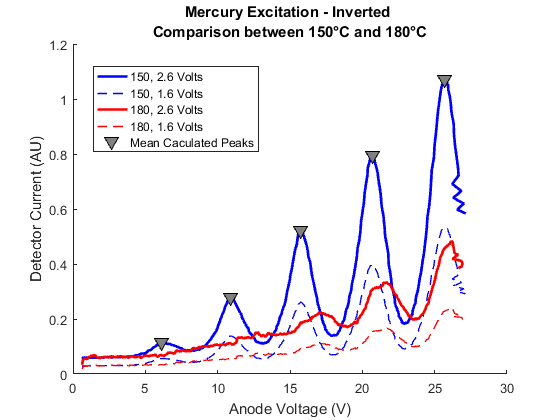
\includegraphics[width = .5\textwidth,keepaspectratio]{peaksmer.png}
\caption{Plot of Current (in arbitrary units) vs. Supplied anode voltage in steps of 80 mV of each experimental run of data, with varying temperature and voltage, and the peak locations found.}
\label{fig:peak2}
\end{figure}
As in the Helium experiment, we  find the peaks in our data by using the \fp\cite{peak} function in Matlab and setting a reasonable prominence cut-off value, we analyze both the peaks and their properties, such as the FWHM values, of the Mercury data. The prominence used for both temperatures of data is 0.02. The values returned are


\begin{center}
\begin{tabular}{c  c  c  } Peak Voltage & $\sigma$ & Difference Between Peaks\\\hline
  6.2332   &$\pm$ 0.1624 &       0      \\
 10.9096  &$\pm$ 0.0903 & 4.6764 \\
  15.7021 &$\pm$ 0.0315 & 4.7925 \\
  20.6838 &$\pm$ 0.0581 & 4.9871 \\                 
  25.7021 &$\pm$ 0.0503 & 5.0183 \\
\end{tabular}
\end{center}

where we've found the difference in the peaks by taking the maximum value of each peak and subtracting it with the peak below it, which gives us a relative spacing between each peak.
If we average the value for the difference between peaks using \textbf{Fig. \ref{eq:mean}} and finding the total error using \textbf{Fig. \ref{eq:quad}}, we find the total error(s) to be

\begin{center}
\begin{tabular}{c  c  c  c }
FWHM &$\sigma_{FWHM}$ & $\sigma_{syst}$ & $\sigma_{final}$\\\hline
1.64 & 0.6964&80 &$\pm$ 0.7151\\
1.58 & 0.6709&80 &$\pm$ 0.6769\\
1.81 & 0.7668&80 &$\pm$0.7674\\
1.79 & 0.7601&80 &$\pm$0.7632\\
\end{tabular}
\end{center}

Finally, we were able to determine the work function of the oxide-coated cathode in the Mercury apparatus, which is observed by the positive offset in the plot. we find this value by a simple calculation, knowing the final excitation approximation and the initial peak height,
\[W_0 =\text{Peak}_1 - E_{exc} =  6.2332\quad eV - 4.8686\quad eV = 1.3646\quad eV\]
where $W_0$ is the work function, Peak$_1$ is the first voltage of the first observed peak and E$_{exc}$ is the estimated excitation energy. Our final results are
\textbf{
\begin{center}
\begin{tabular}{c c c c c }
Measured & $\sigma_{final}$ & Accepted & \% Diff\\\hline
E&$4.87\quad eV$ &$ \pm 1.46\quad eV$ & 4.9 & 0.64\% \\
$W_0$&$1.36\quad eV$ & $\pm .14\quad eV$  & 1.2 & 12.3\%
\end{tabular}
\end{center}}

\subsection{Analysis Summation}
In both experiments, the experimental values calculated for the excitation energy levels are in very good agreement with the accepted values, however, a problem arises when looking at the expected work function vs. the calculated work function. Our value is 12.3\% off of the expected value which suggests either there was a mistake in the calculation, or the accepted work function for this particular oxide-coated cathode is not the same value as the the accepted value used. The dominant factor for errors is clearly systematic errors that arise from the limitations of the Labview software. Because we're only able to take 0.08 V steps, we'll never be able to limit the error to be less than 0.05 V, or half a division.



\section{\label{sec:results}Results and Discussion}
After performing the analysis, our findings agree with excitation and ionization energies we expect to see for Helium and Mercury. The percentage difference between the accepted values and our experimental values are very low as well as the final error calculations. We can say with some degree of confidence that the experiment overall was a success. However, there are some limitations and we can certainly get our errors to be much lower. A significant source of systematic error is the fact that our Labview program only allowed us to take voltage steps of 80 mV. This gives us an absolute minimum error, half a division of 80 V. If we were able to decrease this voltage step, allowing us to take more data points with finer granularity, we would be able to reduce the total error and find a more exact value for the excitation energies. 

\section{\label{sec:results}Conclusion}
By measuring the inelastic collisions between helium/mercury atoms and accelerated electrons, we were able to determine that there are discrete energy levels at which excitation occurs. This is in agreement with the theoretical statement that energy levels are quantized, as proposed by Niels Bohr. This has very important implications because it allows us to study the interactions between various atoms and allows us to classify atoms purely by their discrete excitation levels. With this information, we're able to probe more complex systems (gases, stars, ect.) to determine their compositional makeups, knowing that the atoms that make up the system have quantized energies associated with them, hence, they have a unique signature. If we extend this to systems where we cannot directly observer its composition, we can find energy states of the system that allow us to classify the system. Knowing that atoms have quantized energy states also allows us to further probe the properties of the different ions of atoms and how they might benefit other research.
\begin{figure*}[!hb]\centering
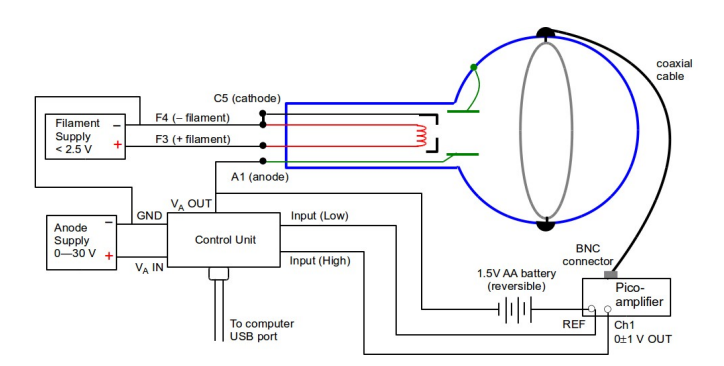
\includegraphics[width = \textwidth,keepaspectratio]{heliumb.png}
\caption{Experimental setup for Helium. Further Details expressed in \textbf{\ref{sec:meth}. Methods: \textit{Helium} }}
\label{fig:helb}
\end{figure*}

\begin{figure*}[!hb]\centering
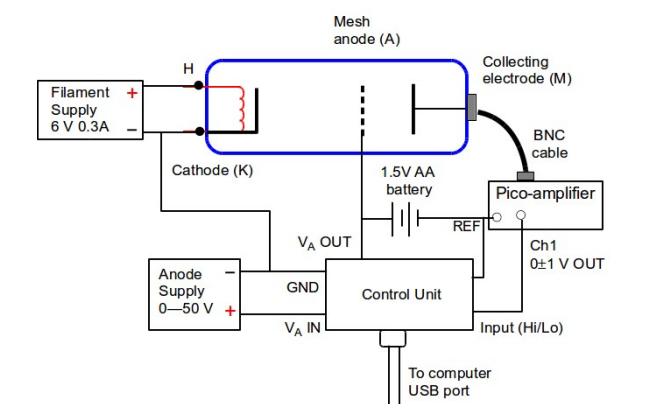
\includegraphics[width = \textwidth,keepaspectratio]{mercuryb.png}
\caption{Experimental setup for mercury. Further Details expressed in \textbf{\ref{sec:meth}. Methods: \textit{Mercury} }}
\label{fig:merb}
\end{figure*}


\begin{thebibliography}{50}
\section{\label{sec:level5}Bibliography}
\bibitem{bohrmodel} \url{https://en.wikipedia.org/wiki/Bohr_model}\\
\bibitem{ruth} E. Rutherford, F.R.S.*
Philosophical Magazine
Series 6, vol. 21
May 1911, p. 669-688
\url{http://www.chemteam.info/Chem-History/Rutherford-1911/Rutherford-1911.html}
\bibitem{ruthmodel} \url{https://en.wikipedia.org/wiki/Rutherford_model}\\%\bibitem{SBH}
\bibitem{esderiv} \url{http://venables.asu.edu/quant/Dinesh/Bohratom2.html}\\
\bibitem{shield} \url{https://en.wikipedia.org/wiki/Shielding_effect}\\
\bibitem{hell} \url{http://www.physics.umanitoba.ca/~mgericke/Teaching/Phys3380/Lectures/Lecture30.pdf}\\
\bibitem{peak} \url{https://www.mathworks.com/help/signal/examples/peak-analysis.html}
\bibitem{qi} \url{https://en.wikipedia.org/wiki/Polynomial_interpolation}
%S B Hosur and N M Badger,
%\textit{Compton shift in energy and wavelength—a laboratory experiment
%}. Am. J. Phys. 55 175\\
\end{thebibliography}

\end{document}
%
% ****** End of file apssamp.tex ******
